\newcommand{\svrname}{Dr John Fawcett}
\newcommand{\jkfside}{oneside}
\newcommand{\jkfhanded}{right}

\newcommand{\studentname}{Harry Langford}
\newcommand{\studentemail}{hjel2@cam.ac.uk}

\documentclass[10pt,\jkfside,a4paper]{article}

\input{./templatenst/includes.tex}
% DO NOT add \usepackage commands here.  Place any custom commands
% into your SV work files.  Anything in the template directory is
% likely to be overwritten!

\usepackage{fancyhdr}

\usepackage{lastpage}       % ``n of m'' page numbering
\usepackage{lscape}         % Makes landscape easier

\usepackage{verbatim}       % Verbatim blocks
\usepackage{epsfig}         % Embed encapsulated postscript
\usepackage{array}          % Array environment
\usepackage[nolinks]{qrcode}         % QR codes
\usepackage{enumitem}       % Required by Tom Johnson's exam question header

\usepackage{hhline}         % Horizontal lines in tables
\usepackage{siunitx}        % Correct spacing of units
\usepackage{amsmath}        % American Mathematical Society
\usepackage{amssymb}        % Maths symbols
\usepackage{amsthm}         % Theorems

\usepackage{ifthen}         % Conditional processing in tex

\usepackage[top=3cm,
            bottom=3cm,
            inner=2cm,
            outer=5cm]{geometry}

% PDF metadata + URL formatting
\usepackage[
            pdfauthor={\studentname},
            pdftitle={\svcourse, SV \svnumber},
            pdfsubject={},
            pdfkeywords={9d2547b00aba40b58fa0378774f72ee6},
            pdfproducer={},
            pdfcreator={},
            hidelinks]{hyperref}

\renewcommand{\headrulewidth}{0.4pt}
\renewcommand{\footrulewidth}{0.4pt}
\fancyheadoffset[LO,LE,RO,RE]{0pt}
\fancyfootoffset[LO,LE,RO,RE]{0pt}
\pagestyle{fancy}
\fancyhead{}
\fancyhead[LO,RE]{{\bfseries \studentname}\\\studentemail}
\fancyhead[RO,LE]{{\bfseries \svcourse, SV~\svnumber}\\\svdate\ \svtime, \svvenue}
\fancyfoot{}
\fancyfoot[LO,RE]{For: \svrname}
\fancyfoot[RO,LE]{\today\hspace{1cm}\thepage\ / \pageref{LastPage}}
\fancyfoot[C]{\qrcode[height=0.8cm]{\svuploadkey}}
\setlength{\headheight}{22.55pt}

\ifthenelse{\equal{\jkfside}{oneside}}{

 \ifthenelse{\equal{\jkfhanded}{left}}{
  % 1. Left-handed marker, one-sided printing or e-marking, use oneside and...
  \evensidemargin=\oddsidemargin
  \oddsidemargin=73pt
  \setlength{\marginparwidth}{111pt}
  \setlength{\marginparsep}{-\marginparsep}
  \addtolength{\marginparsep}{-\textwidth}
  \addtolength{\marginparsep}{-\marginparwidth}
 }{
  % 2. Right-handed marker, one-sided printing or e-marking, use oneside.
  \setlength{\marginparwidth}{111pt}
 }

}{
 % 3. Alternating margins, two-sided printing, use twoside.
}

\setlength{\parindent}{0em}
\addtolength{\parskip}{1ex}

% Exam question headings, labels and sensible layout (courtesy of Tom Johnson)
\setlist{parsep=\parskip, listparindent=\parindent}
\newcommand{\examhead}[3]{\section{#1 Paper #2 Question #3}}
\newenvironment{examquestion}[3]{
    \examhead{#1}{#2}{#3}\setlist[enumerate, 1]{label=(\alph*)}\setlist[enumerate, 2]{label=(\roman*)}
    \marginpar{\qrcode{https://www.cl.cam.ac.uk/teaching/exams/pastpapers/y#1p#2q#3.pdf}}
    \marginpar{\footnotesize \url{https://www.cl.cam.ac.uk/teaching/exams/pastpapers/y#1p#2q#3.pdf}}
}{}



\fancyhead[RO,LE]{{\bfseries NST Maths, Easter~Work}}

\usepackage{physics}
\usepackage{enumitem}
\usepackage{graphicx}
\graphicspath{ {./images/} }
\usepackage{tikz}

\begin{document}

\section*{Fourier Series}

\begin{enumerate}

\setcounter{enumi}{20}

\item 

\[
\begin{split}
 & \int^1_{-1} 1 \times x \dd{x} \\
=& \int^1_{-1} x \dd{x} \\
=& \left[\frac{1}{2}x^2 \right]^1_{-1} \\
=& \frac{1}{2} - \frac{1}{2} \\
=& 0 \\
\end{split}
\]
So $1$ is orthogonal to $x$ on the interval $[-1, 1]$.

\[
\begin{split}
 & \int^1_{-1} 1 \times \frac{1}{2}(3x^2 - 1) \dd{x} \\
=& \int^1_{-1} \frac{1}{2}(3x^2 - 1) \dd{x} \\
=& \left[\frac{1}{2}(x^3 - x) \right]^1_{-1} \\
=& 0 - 0 \\
=& 0 \\
\end{split}
\]
So $1$ is orthogonal to $\frac{1}{2}(3x^2 - 1)$ on the interval $[-1, 1]$.

\[
\begin{split}
 & \int^1_{-1} 1 \times \frac{1}{2}(5x^3 - 3x) \dd{x} \\
=& \int^1_{-1} \frac{1}{2}(5x^3 - 3x) \dd{x} \\
=& \left[\frac{1}{8}(5x^4 - 6x^2) \right]^1_{-1} \\
=& -\frac{1}{8} - - \frac{1}{8} \\
=& 0 \\
\end{split}
\]
So $1$ is orthogonal to $\frac{1}{2}(5x^3 - 3x)$ on the interval $[-1, 1]$.

\[
\begin{split}
 & \int^1_{-1} x \times \frac{1}{2}(3x^2 - 1) \dd{x} \\ 
=& \int^1_{-1} \frac{1}{2}(3x^3 - x) \dd{x} \\
=& \left[ \frac{1}{8}(3x^4 - 2x^2) \right]^1_{-1} \\
=& \frac{1}{8} - \frac{1}{8} \\
=& 0 \\
\end{split}
\]
So $x$ is orthogonal to $\frac{1}{2}(3x^2 - 1)$ on the interval $[-1, 1]$.

\[
\begin{split}
 & \int^1_{-1} x \times \frac{1}{2}(5x^3 - 3x) \dd{x} \\
=& \int^1_{-1} \frac{1}{2}(5x^4 - 3x^2) \dd{x} \\
=& \left[\frac{1}{2}(x^5 - x^2)\right]^1_{-1} \\
=& 0 - 0 \\
=& 0 \\
\end{split}
\]
So $x$ is orthogonal to $\frac{1}{2}(5x^3 - 3x)$ on the interval $[-1, 1]$.

\[
\begin{split}
 & \int^1_{-1} \frac{1}{2}(3x^2 - 1) \times \frac{1}{2}(5x^3 - 3x) \dd{x} \\
=& \int^1_{-1} \frac{1}{4}(15x^5 - 14x^3 + 3x) \dd{x} \\
=& \left[ \frac{1}{8}(5x^6 - 7x^4 + 3x^2) \right]^1_{-1} \\
=& \frac{1}{8} - \frac{1}{8} \\
=& 0 \\
\end{split}
\]
So $\frac{1}{2}(3x^2 - 1)$ is orthogonal to $\frac{1}{2}(5x^3 - 3x)$ on the interval $[-1, 1]$.

So the functions $1$, $x$, $\frac{1}{2}(3x^2 - 1)$ and $\frac{1}{2}(5x^3 - 3x)$ are orthogonal 
on the interval $[-1, 1]$.

\item 

\[
\begin{split}
 & \int^a_0 \sin(mx)\sin(nx) \dd{x} \\
=& \frac{1}{2}\int^a_0 \cos((m - n)x) - \cos((m + n)x) \dd{x} \\
=& \frac{1}{2}\left[ \frac{1}{m - n}\sin((m - n)x) - \frac{1}{m + n}\sin((m + n)x) \right]^a_0 \\
=& \frac{1}{2}\left( \frac{1}{m - n}\sin((m - n)k\pi) - \frac{1}{m + n}\sin((m + n)k\pi) - \frac{1}{m - n}\sin 0 + \frac{1}{m + n}\sin 0 \right) \\
=& \frac{1}{2}\times 0 \\
=& 0 \\
\end{split}
\]

\item 

For $m \neq n$:

\[
\begin{split}
 & \int^T_{-T} \sin\left(\frac{m\pi\theta}{T}\right)\sin\left(\frac{n\pi\theta}{T}\right) \dd{\theta} \\
=& \frac{1}{2}\int^T_{-T} \cos\left(\frac{(m - n)\pi\theta}{T}\right) - \cos\left(\frac{(m + n)\pi\theta}{T}\right) \dd{\theta} \\
=& \frac{1}{2}\left[ \frac{T}{(m - n)\pi}\sin\left(\frac{(m - n)\pi\theta}{T}\right) - \frac{T}{(m + n)\pi}\sin\left(\frac{(m + n)\pi\theta}{T}\right) \right]^T_{-T} \\
=& \frac{1}{2}\left( \frac{T}{(m - n)\pi}\left(\sin\left((m - n)\pi\right) - \sin\left(-(m - n)\pi\right)\right) - \frac{T}{(m + n)\pi}\left(\sin\left((m + n)\pi\right) - \sin\left(-(m + n)\pi\right) \right)\right) \\
=& \frac{1}{2}\left( 0 \right) \\
=& 0 \\
\end{split}
\]

For $m = n$:

\[
\begin{split}
 & \int^T_{-T} \sin\left(\frac{m\pi\theta}{T}\right)\sin\left(\frac{n\pi\theta}{T}\right) \dd{\theta} \\
=& \int^T_{-T} \sin^2\left(\frac{n\pi\theta}{T}\right) \dd{\theta} \\
=& \frac{1}{2}\int^T_{-T} 1 - \cos\left(\frac{2n\pi\theta}{T}\right) \dd{\theta} \\
=& \frac{1}{2}\left[ \theta - \frac{T}{2n\pi}\sin\left(\frac{2n\pi\theta}{T}\right) \right]^T_{-T} \\
=& \frac{1}{2}\left(T - 0 - - T + 0\right) \\
=& T \\
\end{split}
\]

\item 

\[
\sin2\theta = \sin2\theta \\
\]

\[
\cos^2\theta = \frac{1}{2} - \frac{1}{2}\cos2\theta \\
\]

\[
\sin^3\theta = \frac{3}{4}\sin\theta - \frac{1}{4}\sin3\theta \\
\]

\item 

Note that $|x|$ is an even function and the period is $\ell$, so the Fourier Series 
is of the form $a_0 + \sum^\infty_{i=1}\cos\left(\frac{i\pi x}{\ell}\right)$.

The constant is given by:
\[
\begin{split}
a_0 =& \int^\ell_{-\ell} |x| \dd{x} \\
=& \frac{2}{\ell}\int^\ell_0 x \dd{x} \\
=& \frac{2}{\ell}\left[ \frac{1}{2}x^2 \right]^\ell_0 \\
=& \ell \\
\end{split}
\]

The coefficients $a_i$ are given by:
\[
\begin{split}
a_n &= \frac{1}{\ell}\int^\ell_{-\ell} |x|\cos\left(\frac{n\pi x}{\ell}\right) \dd{x} \\
&= \frac{2}{\ell}\int^\ell_0 x\cos\left(\frac{n\pi x}{\ell}\right) \dd{x} \\
&= \frac{2}{\ell}\left[ \frac{\ell}{n\pi}x\sin\left(\frac{n\pi x}{\ell}\right) + \left(\frac{\ell}{n\pi}\right)^2\cos\left(\frac{n\pi x}{\ell}\right)\right]^\ell_0 \\
&= \frac{2}{\ell}\left( \frac{\ell}{n\pi}x\sin\left(n\pi\right) + \left(\frac{\ell}{n\pi}\right)^2\cos\left(n\pi\right) - \frac{\ell}{n\pi}x\sin 0 - \left(\frac{\ell}{n\pi}\right)^2\cos 0\right) \\
&= \frac{2}{\ell}\left(\frac{\ell}{n\pi}\right)^2\left(\cos\left(n\pi\right) - 1\right) \\
a_n &= 
\begin{cases}
0 & \text{if } n \% 2 = 0 \\
-\frac{4\ell}{(n\pi)^2} & \text{if } n \% 2 = 1 \\
\end{cases}
\end{split}
\]

So the Fourier Series for the function that equals $|x|$ when $\ell \leq x \leq \ell$ and 
is periodic with period $2\ell$ is equal to:

\[
\begin{split}
f(x) &= \frac{a_0}{2} + \sum^\infty_{n=1}a_n\cos(nx) \\
f(x) &= \frac{\ell}{2} - \frac{4\ell}{\pi^2}\sum^\infty_{n=0} \frac{\cos\left(\frac{(2n + 1)\pi x}{\ell}\right)}{(2n + 1)^2} \\
\end{split}
\]

If the series is integrated then the resulting series will sum to $\int |x| \dd{x}$.

\begin{center}
\includegraphics[width=5cm]{sv15integral}
\end{center}

If the series is differentiated then the resulting series will sum to $\dv{x} |x|$. This is 
$-1$ if $x < 0$ and $1$ if $x > 0$.

\begin{center}
\includegraphics[width=5cm]{sv15derivative}
\end{center}

\item 
\begin{enumerate}

\item 
\[
\begin{split}
a_0 &= \frac{1}{\pi}\int^\pi_{-\pi}e^x \dd{x} \\
&= \frac{1}{\pi}\left[e^x \right]^\pi_{-\pi} \\
&= \frac{1}{\pi}\left(e^\pi - e^{-\pi}\right) \\
\end{split}
\]

\[
\begin{split}
\int e^x\cos(nx)\dd{x} &= e^x\cos(nx) + n\int e^x\sin(nx) \dd{x} \\
\int e^x\sin(nx)\dd{x} &= e^x\sin(nx) - n\int e^x\cos(nx) \dd{x} \\
\int e^x\cos(nx)\dd{x} &= e^x\cos(nx) + ne^x\sin(nx) - n^2\int e^x\cos(nx) \dd{x} \\
(n^2 + 1)\int e^x\cos(nx)\dd{x} &= e^x\cos(nx) + ne^x\sin(nx) \\
\int e^x\cos(nx)\dd{x} &= \frac{1}{n^2 + 1}(e^x\cos(nx) + ne^x\sin(nx)) \\
\int e^x\sin(nx)\dd{x} &= e^x\sin(nx) - ne^x\cos(nx) - n^2\int e^x\sin(nx) \dd{x} \\
(n^2 + 1)\int e^x\sin(nx)\dd{x} &= e^x\sin(nx) - ne^x\cos(nx) \\
\int e^x\sin(nx)\dd{x} &= \frac{1}{n^2 + 1}(e^x\sin(nx) - ne^x\cos(nx)) \\
\end{split}
\]

\[
\begin{split}
a_n &= \frac{1}{\pi}\int^\pi_{-\pi} e^x \cos\left(nx\right) \dd{x} \\
    &= \frac{1}{(n^2 + 1)\pi}\left[e^x\cos(nx) + ne^x\sin(nx)\right]^\pi_{-\pi} \\
	&= \frac{1}{(n^2 + 1)\pi}\left(e^{\pi}\cos(n\pi) - e^{-\pi}\cos(n\pi)\right) \\
	&= \frac{(-1)^n(e^{\pi} - e^{-\pi})}{(n^2 + 1)\pi} \\
\end{split}
\]

\[
\begin{split}
b_n &= \frac{1}{\pi}\int^\pi_{-\pi} e^x\sin(nx) \dd{x} \\
	&= \frac{1}{(n^2 + 1)\pi}[e^x\sin(nx) - ne^x\cos(nx)]^\pi_{-\pi} \\
	&= \frac{1}{(n^2 + 1)\pi}(-ne^\pi\cos(n\pi) + ne^{-\pi}\cos(n\pi)) \\
	&= \frac{(-1)^{n+1}n(e^\pi - e^{-\pi})}{(n^2 + 1)\pi} \\
\end{split}
\]

\[
f(x) = \frac{e^\pi - e^{-\pi}}{\pi}\left(\frac{1}{2} + \sum^\infty_{n=1}\frac{(-1)^n}{n^2 + 1}(\cos(nx) - n\sin(nx))\right) \\
\]

When $x = \pi$ and $x = -\pi$, $f(x)$ converges to $\frac{e^\pi + e^{-\pi}}{2}$.

\item 

Given an arbitrary function $f$ defined for a range $[-a, a]$ where $a$ is a 
(possibly infinite) real.

Consider the functions defined over the range $[-a, a]$:
\[
\begin{split}
f_e(x) &\triangleq \frac{1}{2}(f(x) + f(-x)) \\
f_o(x) &\triangleq \frac{1}{2}(f(x) - f(-x)) \\
\end{split}
\]

\[
\begin{split}
f_e(x) &= \frac{1}{2}(f(x) + f(-x)) \\
	   &= \frac{1}{2}(f(-x) + f(x)) \\
	   &= f_e(-x) \\
\end{split}
\]
So $f_e(x)$ is an even function.

\[
\begin{split}
f_o(x) &= \frac{1}{2}(f(x) - f(-x)) \\
	   &= -\frac{1}{2}(f(-x) - f(x)) \\
	   &= -f(-x) \\
\end{split}
\]
So $f_o(x)$ is an odd function.

\[
\begin{split}
f_e(x) f_o(x) &= \frac{1}{2}(f(x) + f(-x)) + \frac{1}{2}(f(x) - f(-x)) \\
			  &= f(x) \\
\end{split}
\]

So given an arbitrary function $f$ we hve constructed an even function $f_e$ and an odd 
function $f_o$ such that $f = f_e + f_o$.

Hence any function $f(x)$ can be written as the sum of an even function and an odd function.

\vspace{0.5cm}

\[
\begin{split}
\cosh(x) &= \frac{e^x + e^{-x}}{2} \\
		 &= \frac{e^\pi - e^{-\pi}}{2\pi}\left(\frac{1}{2} + \sum^\infty_{n=1}\frac{(-1)^n}{n^2 + 1}(\cos(nx))\right) \\
\end{split}
\]

\[
\begin{split}
\sinh(x) &= \frac{e^x - e^{-x}}{2} \\
		 &= -\frac{e^\pi - e^{-\pi}}{\pi}\left(\sum^\infty_{n=1}\frac{(-1)^n}{n^2 + 1}(n\sin(nx))\right)
\end{split}
\]

\end{enumerate}

\item 

\[
\begin{split}
 & \int^\pi_{-\pi} f(x)g(x) \dd{x} \\
=& \int^\pi_{-\pi} \sum^\infty_{n=1}b_n\cos(nx)\sum^\infty_{m=1}B_m\sin(mx) \dd{x} \\
=& \sum^\infty_{n=1}\sum^\infty_{m=1}b_nB_m\int^\pi_{-\pi}\sin(mx)\cos(nx) \dd{x} \\
=& \sum^\infty_{n=1}\sum^\infty_{m=1}b_nB_m\delta_{mn}\pi \text{ using (23)} \\
=& \pi\sum^\infty_{n=1}\sum^\infty_{m=1}b_nB_n \\
\end{split}
\]

\[
\begin{split}
 & \int^\pi_{-\pi} f(x)g(x) \dd{x} \\
=& \frac{a_0^2}{4} + \pi\sum^\infty_{n=1}(a^2_n + b^2_n) \\
\end{split}
\]

\item 

\begin{enumerate}

\item \label{fxequalsfminusx} $f(x) = f(-x) \Longrightarrow \forall n \in \mathbb{N}. b_n = 0$

\[
\begin{split}
a_n\cos(nx) + b_n\sin(nx) &= a_n\cos(-nx) + b_n\sin(-nx) \\
a_n\cos(nx) + b_n\sin(nx) &= a_n\cos(nx) + -b_n\sin(nx) \\
a_n = a_n &\wedge b_n = -b_n \\
a_n = a_n &\wedge b_n = 0 \\
\end{split}
\]

\item $f(x) = -f(-x) \Longrightarrow \forall n \in \mathbb{N}. a_n = 0$

\[
\begin{split}
a_n\cos(nx) + b_n\sin(nx) &= -(a_n\cos(-nx) + b_n\sin(-nx)) \\
a_n\cos(nx) + b_n\sin(nx) &= -a_n\cos(nx) + b_n\sin(nx) \\
a_n = -a_n &\wedge b_n = b_n \\
a_n = 0 &\wedge b_n = 0 \\
\end{split}
\]

\item $f(x) = f(\pi - x) \Longrightarrow \forall n \in \mathbb{N}. (n \equiv_2 1 \Longrightarrow a_n = b_n = 0)$

\[
\begin{split}
a_n\cos(nx) + b_n\sin(nx) &= a_n\cos(n\pi - nx) + b_n\sin(n\pi - nx) \\
a_n\cos(nx) + b_n\sin(nx) &= a_n(\cos(n\pi)\cos(nx) - \sin(n\pi)\sin(nx)) + b_n(\cos(n\pi)\sin(nx) - \sin(n\pi)\cos(nx)) \\
a_n\cos(nx) + b_n\sin(nx) &= \cos(n\pi)(a_n\cos(nx) + b_n\sin(nx)) \\
a_n\cos(nx) + b_n\sin(nx) &= (-1)^n(a_n\cos(nx) + b_n\sin(nx)) \\
\end{split}
\]

So if $n$ is odd then $a_n = b_n = 0$.

\item $f(x) = -f(\pi - x) \Longrightarrow \forall n \in \mathbb{N}. (n \equiv_2 0 \Longrightarrow a_n = b_n = 0)$

\[
\begin{split}
a_n\cos(nx) + b_n\sin(nx) &= -(a_n\cos(n\pi - nx) + b_n\sin(n\pi - nx)) \\
a_n\cos(nx) + b_n\sin(nx) &= -(a_n(\cos(n\pi)\cos(nx) - \sin(n\pi)\sin(nx)) + b_n(\cos(n\pi)\sin(nx) - \sin(n\pi)\cos(nx))) \\
a_n\cos(nx) + b_n\sin(nx) &= -\cos(n\pi)(a_n\cos(nx) + b_n\sin(nx)) \\
a_n\cos(nx) + b_n\sin(nx) &= (-1)^{n+1}(a_n\cos(nx) + b_n\sin(nx)) \\
\end{split}
\]

So if $n$ is even then $a_n = b_n = 0$.

\item $f(x) = f\left(\frac{\pi}{2} + x\right) \Longrightarrow \forall n \in \mathbb{N}. (n \% 4 \neq 0 \Longrightarrow a_n = b_n = 0)$

\[
\begin{split}
a_n\cos(nx) + b_n\sin(nx) &= a_n\cos\left(\frac{\pi n}{2} + nx\right) + b_n\sin\left(\frac{\pi n}{2} + nx\right) \\
a_n\cos(nx) + b_n\sin(nx) &= a_n\left(\cos\left(\frac{\pi n}{2}\right)\cos(nx) - \sin\left(\frac{\pi n}{2}\right)\sin(nx)\right) + b_n\left(\sin\left(\frac{\pi n}{2}\right)\cos(nx) +  \cos\left(\frac{\pi n}{2}\right)\sin(nx)\right) \\
a_n\cos(nx) + b_n\sin(nx) &= \left(a_n\cos\left(\frac{\pi n}{2}\right) + b_n\sin\left(\frac{\pi n}{2}\right)\right)\cos(nx) + \left(b_n\cos\left(\frac{\pi n}{2}\right) - a_n\sin\left(\frac{\pi n}{2}\right)\right)\sin(nx) \\
\end{split}
\]

Equating the coefficients of $\cos(nx)$ and $\sin(nx)$ gives:

\[
\begin{split}
a_n &= a_n\cos\left(\frac{\pi n}{2}\right) + b_n\sin\left(\frac{\pi n}{2}\right) \\
b_n &= b_n\cos\left(\frac{\pi n}{2}\right) - a_b\sin\left(\frac{\pi n}{2}\right) \\
\end{split}
\]

Considering the four cases of $n$ \% 4:
\begin{center}
\begin{tabular}{c|c|c|c}
\multicolumn{4}{c}{n \% 4} \\
\hline 
0 & 1 & 2 & 3 \\
\hline
$a_n = a_b$ & $a_n = b_n$ & $a_n = -a_n$ & $a_n = -b_n$ \\
$b_n = b_n$ & $b_n = -a_n$ & $b_n = -b_n$ & $b_n = a_n$ \\
\end{tabular}
\end{center}

$n \equiv_4 1$, $n \equiv_4 2$ and $n \equiv_4 3$ all imply $a_n = -a_n$, $b_n = -b_n$ which implies 
that $a_n = b_n = 0$.

So if $n \% 4 \neq 0$ then $a_n = b_n = 0$.

\item \label{pi2minusx} $f(x) = f\left(\frac{\pi}{2} - x\right) \Longrightarrow \forall n \in \mathbb{N}. (n \% 4 \neq 0 \Longrightarrow a_n = b_n = 0)$

\[
\begin{split}
a_n\cos(nx) + b_n\sin(nx) &= a_n\cos\left(\frac{\pi n}{2} - nx\right) + b_n\sin\left(\frac{\pi n}{2} - nx\right) \\
a_n\cos(nx) + b_n\sin(nx) &= a_n\left(\cos\left(\frac{\pi n}{2}\right)\cos(nx) + \sin\left(\frac{\pi n}{2}\right)\sin(nx)\right) +  b_n\left(\cos\left(\frac{\pi n}{2}\right) - b_n\sin\left(\frac{\pi n}{2}\right)\right)\cos(nx) \\
a_n\cos(nx) + b_n\sin(nx) &= \left(a_n\cos\left(\frac{\pi n}{2}\right) - b_n\sin\left(\frac{\pi n}{2}\right)\right)\cos(nx) + a_n\left(\sin\left(\frac{\pi n}{2}\right) +  b_n\cos\left(\frac{\pi n}{2}\right)\right)\sin(nx) \\
\end{split}
\]

Equating the coefficients of $\cos(nx)$ and $\sin(nx)$ gives:

\[
\begin{split}
a_n &= a_n\cos\left(\frac{\pi n}{2}\right) - b_n\sin\left(\frac{\pi n}{2}\right) \\
b_n &= a_n\sin\left(\frac{\pi n}{2}\right) + b_n\cos\left(\frac{\pi n}{2}\right) \\
\end{split}
\]

Considering the four cases of $n$ \% 4:
\begin{center}
\begin{tabular}{c|c|c|c}
\multicolumn{4}{c}{n \% 4} \\
\hline 
0 & 1 & 2 & 3 \\
\hline
$a_n = a_b$ & $a_n = -b_n$ & $a_n = -a_n$ & $a_n = b_n$ \\
$b_n = b_n$ & $b_n = a_n$ & $b_n = -b_n$ & $b_n = -a_n$ \\
\end{tabular}
\end{center}

$n \equiv_4 1$, $n \equiv_4 2$ and $n \equiv_4 3$ all imply $a_n = -a_n$, $b_n = -b_n$ which implies 
that $a_n = b_n = 0$.

So if $n \% 4 \neq 0$ then $a_n = b_n = 0$.

\item $f(x) = f(2x) \Longrightarrow \forall n \in \mathbb{Z}^+. a_n = b_n = 0$

Note that this restriction is placed on $n \in \mathbb{Z}^+$ -- so $a_0$ is not restricted.

\[
a_n\cos(nx) + b_n\sin(nx) = a_n\cos(2nx) + b_n\sin(2nx) \\
\]

For $n \neq 0$, consider $x = \frac{\pi}{4n}$.

\[
\begin{split}
a_n\cos\left(\frac{\pi}{4}\right) + b_n\sin\left(\frac{\pi}{4}\right) &= a_n\cos\left(\frac{\pi}{2}\right) + b_n\sin\left(\frac{\pi}{2}\right) \\
a_n\frac{\sqrt{2}}{2} + b_n\frac{\sqrt{2}}{2} &= 0 + b_n \\
a_n &= b_n(\sqrt{2} - 1) \\
\end{split}
\]

For $n \neq 0$, consider $x = \frac{3\pi}{4n}$.

\[
\begin{split}
a_n\cos\left(\frac{3\pi}{4}\right) + b_n\sin\left(\frac{3\pi}{4}\right) &= a_n\cos\left(\frac{3\pi}{2}\right) + b_n\sin\left(\frac{3\pi}{2}\right) \\
-a_n\frac{\sqrt{2}}{2} + b_n\frac{\sqrt{2}}{2} &= 0 + -b_n \\
a_n &= b_n(\sqrt{2} + 1) \\
\end{split}
\]

Equating these gives:
\[
\begin{split}
b_n(\sqrt{2} + 1) &= b_n(\sqrt{2} - 1) \\
b_n &= -b_n \\
b_n &= 0 \\
\end{split}
\]
\[
\begin{split}
a_n &= b_n(\sqrt{2} - 1) \\
a_n &= 0 \\
\end{split}
\]

So for $n \neq 0$, $a_n = b_n = 0$.

\item $f(x) = f(-x) = f\left(\frac{\pi}{2} - x\right) \Longrightarrow \forall n \in \mathbb{N}. b_n = 0 \wedge (n \% 4 \neq 0 \Longrightarrow a_n = b_n = 0)$

\[
\begin{split}
f(x) = f(-x) = f\left(\frac{\pi}{2} - x\right) &\Longleftrightarrow \\
f(x) = f(-x) \wedge f(x) = f\left(\frac{\pi}{2} - x\right) \wedge f(-x) = f\left(\frac{\pi}{2} - x\right) &\Longleftrightarrow \\
f(x) = f(-x) \wedge f(x) = f\left(\frac{\pi}{2} - x\right) \wedge f(x) = f\left(\frac{\pi}{2} - x\right) & \text{ using } f(x) = f(-x) \Longleftrightarrow \\
f(x) = f(-x) \wedge f(x) = f\left(\frac{\pi}{2} - x\right)& \\
\end{split}
\]

This reduces the problem down to two problems both of which we have already solved.

So $\forall n \in \mathbb{N}. b_n = 0$ and if $n \% 4 \neq 0$ then $a_n = 0$.

\end{enumerate}

\item 

\[
\begin{split}
\sum^\infty_{-\infty}c_ne^{inx} &= x^2 \\
\sum^\infty_{-\infty}c_ne^{inx}e^{-imx} &= x^2e^{-imx} \\
\sum^\infty_{-\infty}c_n\int^\pi_{-\pi}e^{inx}e^{-imx} \dd{x} &= \int^\pi_{-\pi}x^2\cos(mx) \dd{x} \\
\sum^\infty_{-\infty}2\pi \delta_{mn}c_n &= \left[\frac{1}{m}x^2\sin(mx) + \frac{2}{m^2}x\cos(mx) - \frac{2}{m^3}\sin(mx)\right]^\pi_{-\pi} \\
2\pi c_m &= \left[\frac{2}{m^2}x\cos(mx)\right]^\pi_{-\pi} \\
2\pi c_m &= \frac{4\pi}{m^2}\cos(m\pi) \\
c_m &= \frac{2}{m^2}\cos(m\pi) \\
c_m &= (-1)^m\frac{2}{m^2} \\
\end{split}
\]

Consider $a_0$:
\[
\begin{split}
a_0 &= \frac{1}{\pi}\int^\pi_{-\pi} x^2 \dd{x} \\
a_0 &= \frac{2}{3\pi}\left[ x^3 \right]^\pi_0 \\
a_0 &= \frac{2\pi^2}{3} \\
\end{split}
\]

Combining the above results gives:
\[
x^2 = \frac{2\pi^2}{3 \times 2} + \sum^\infty_{-\infty} (-1)^m \frac{2}{m^2}\cos(mx)
\]

\item 

\begin{enumerate}

\item 

The \textit{odd} function which is periodic with period $2\pi$ and equal to $f(x)$ for 
$0 \leq x \leq pi$:

\begin{center}
\begin{tikzpicture}[scale=0.5]
\draw[help lines, color=gray!30, dashed] (-3.9,-3.9) grid (3.9,3.9);
\draw[-stealth, thick] (-4.1,0)--(4.1, 0) node[right] {$x$};
\draw[-stealth, thick] (0, -4.1)--(0, 4.1) node[above] {$y$};
\draw (-3.9, 2.3831853071795863) -- (-3.141592653589793, 3.141592653589793);
\draw (-3.141592653589793, 3.141592653589793) -- (-3.141592653589793, -3.141592653589793);
\draw (-3.141592653589793, -3.141592653589793) -- (3.141592653589793, 3.141592653589793);
\draw (3.141592653589793, 3.141592653589793) -- (3.141592653589793, -3.141592653589793);
\draw (3.141592653589793, -3.141592653589793) -- (3.9, -2.3831853071795863);
\end{tikzpicture}
\end{center}

\item 

The \textit{even} function which is periodic with period $2\pi$ and equal to $f(x)$ for 
$0 \leq x \leq pi$.

\begin{center}
\begin{tikzpicture}[scale=0.5]
\draw[help lines, color=gray!30, dashed] (-3.9,-3.9) grid (3.9,3.9);
\draw[-stealth, thick] (-4.1,0)--(4.1, 0) node[right] {$x$};
\draw[-stealth, thick] (0, -4.1)--(0, 4.1) node[above] {$y$};
\draw (-3.9, 2.3831853071795863) -- (-3.141592653589793, 3.141592653589793);
\draw (-3.141592653589793, 3.141592653589793) -- (0, 0);
\draw (0, 0) -- (3.141592653589793, 3.141592653589793);
\draw (3.141592653589793, 3.141592653589793) -- (3.9, 2.3831853071795863);
\end{tikzpicture}
\end{center}

\end{enumerate}

If the function is odd then $\forall n \in \mathbb{N}. a_n = 0$.

\[
\begin{split}
b_n &= \frac{1}{\pi}\int^\pi_{-\pi}x\sin(nx)\dd{x} \\
b_n &= \frac{1}{\pi}\left[-\frac{x}{n}\cos(nx) + \frac{1}{n^2}\sin(nx) \right]^\pi_{-\pi} \\
b_n &= \frac{1}{\pi}\left(-\frac{\pi}{n}\cos(n\pi) + \frac{1}{n^2}\sin(n\pi) - \frac{\pi}{n}\cos(n\pi) + \frac{1}{n^2}\sin(n\pi) \right) \\
b_n &= -\frac{2}{n}\cos(n\pi) \\
b_n &= 2\frac{(-1)^{n+1}}{n} \\
\end{split}
\]

So:
\[
\begin{split}
f(x) &= \sum^\infty_0 2\frac{(-1)^{n+1}}{n} \\
f(x) &= 2\sum^\infty_0 \frac{(-1)^{n+1}}{n} \\
\end{split}
\]
As required.

If the function is even then $\forall n \in \mathbb{N}. b_n = 0$.

\[
\begin{split}
a_0 &= \frac{1}{\pi}\int^\pi_{-\pi} |x| \dd{x} \\
a_0 &= \frac{2}{\pi}\int^\pi_0 x \dd{x} \\
a_0 &= \frac{2}{\pi}\left[\frac{1}{2}x^2 \right]^\pi_0 \\
a_0 &= \pi \\
\end{split}
\]

\[
\begin{split}
a_n &= \frac{1}{\pi} \int^\pi_{-\pi} |x|\cos(nx) \dd{x} \\
a_n &= \frac{2}{\pi} \int^\pi_0 x\cos(nx) \dd{x} \\
a_n &= \frac{2}{\pi} \left[ \frac{x}{n}\sin(nx) + \frac{1}{x^2}\cos(nx) \right]^\pi_0 \\
a_n &= \frac{2}{\pi} \left(\frac{1}{n^2}\cos(n\pi) - \frac{1}{n^2}\right) \\
a_n &= \frac{2}{\pi n^2}(\cos(n\pi) - 1) \\
a_n &= \begin{cases}
0 & \text{if } n \% 2 = 0 \\
-\frac{4}{\pi n^2} & \text{if } n \% 2 = 1 \\
\end{cases}
\end{split}
\]

\[
\sum^\infty_{n=1} a_n = \sum^\infty_{k=0} a_{2k+1} \\
\]

So:
\[
\begin{split}
f(x) &= \frac{\pi}{2} + \sum^\infty_{k=0} -\frac{4}{\pi (2k + 1)^2} \cos(2k+1)x \\
f(x) &= \frac{\pi}{2} - \frac{4}{\pi}\sum^\infty_{k=0} \frac{\cos(2k+1)x}{(2k + 1)^2} \\
\end{split}
\]
As required.

\end{enumerate}

\end{document}